\chapter{System Results}
\label{system-results}

\section{Development}
\subsection{Frameworks and Environments}
RadGrad was built using the Meteor JavaScript web framework. Meteor is integrated with MongoDB and uses the Distributed Data Protocol and publish-subscribe pattern to create real time, responsive code that automatically updates data changes to the client. On the client side, RadGrad uses jQuery and Semantic UI to design and create the user interface. Due to excellent Meteor integration, RadGrad was developed using IntelliJ IDEA. In an effort to create clean and uniform code, RadGrad uses ESLint to confrom to the AirBnB Javascript Style Guide. 

\subsection{Project Management}


\section{Data Model}
\subsection{Career Goals}
Career goals represent possible ICS related careers that ICS students can aspire to get after graduation. Each career goal has an associated name, slug, description, related interests, and an optional URL for more information. Students can choose as many career goals as they want. Faculty and mentors can choose career goals that they would like to be associated with as well.  

\begin{table}[h!]
\centering
\begin{tabular}{ l l l } 
 Data Scientist & Database Administrator & DevOps Engineer \\ 
 Full Stack Developer & Game Developer & Graduate School \\ 
 Information Security Analyst & Information System Manager & IoT Architect \\ 
 Mobile App Developer & Network Engineer & Research Scientist \\
 Robotics Engineer & Software Developer & Startup Co-Founder \\
 Teacher & UX Designer & VR/AR Engineer 
\end{tabular}
\caption{List of RadGrad career goals as of April 2017}
\label{table:1}
\end{table}

\subsection{Courses}
Courses represent all past, present, and future ICS courses. Each course has an associated name, short name, slug, course number, description, credit hours, related interests, a syllabus URL, a URL for more information, and associated prerequisites. The course name is the official name appearing in the UH registration guide, and the course short name is used for display purposes. Students may add as many courses as they would like to their degree plan. 

Course instances represent individual instances for each student. Each course instance has an associated semester, course, whether it has been verified or not, whether it came from STAR or not, grade, credit hours, note, student, and associated ICE points. A course instance is considered verified if ???. A course instance has a note if it is not an ICS course. It is important to note that course instances on RadGrad are only valid on RadGrad, and students must use other methods to officially make UH course registration changes.

\subsection{Desired Degrees}
Desired degrees represent all past, present, and future ICS degrees. Each desired degree has an associated name, short name, slug, and description. Students can only choose one desired degree at any given time. However, they are free to switch desired degrees as many times as they want. It is important to note that desired degrees on RadGrad are only valid on RadGrad, and students must use other methods to officially change their declared degree at UH. 

\subsection{Degree Programs}
Degrees programs represent all past, present, and future ICS degree programs.

\subsection{Feeds}
Feeds represent select actions of RadGrad users. Each feed has associated users, opportunity, course, semester, description, time stamp of the action, picture, and feed type. A feed could have one or multiple users. There are currently six different feed types: a new RadGrad user is added, a new course is added to RadGrad, a new opportunity is added to RadGrad, a user has been verified for completing an opportunity, a new course review has been added, and a new opportunity review has been added. These particular actions have been selected because they could be useful and of interest to other RadGrad users.

\subsection{Feedbacks}
Feedbacks represent recommendations and warnings for students. Each feedback has an associated name, slug, description, and feedback type. There are currently two feedback types: recommendation and warning. 

Feedback instances represent individual instances for each student. Each feedback instance has an associated feedback, user, description, and area. There are currently four different areas: interests, ICE, STAR, and degree plan. Each time the student's plan changes, feedback instances in these areas are deleted and recalculated.

\subsection{Help Messages}
Help messages represent guidance for a particular RadGrad page. Each help message has an associated route name, title, and text. The text can contain actual text, images, and formatting. Each page (route name) can have at most one help message. These help messages are displayed at the top of the specified page, in a collapsible pane.  

%% insert help message image here

\subsection{ICE}
ICE represents a student's ICE points. Each ICE has an associated number for ``I", ``C", and ``E." There are two types of ICE points: earned and planned. Earned ``I" and ``E" points are calculated by adding the ``I" or ``E" points for each verified opportunity in the student's plan. Earned ``C" points are calculated by adding the ``C" points for each verified course in the student's plan. The amount of earned points for each course depends on the grade that the student received; A's represent more points than B's. Planned ``I" and ``E" points are calculated by adding the ``I" or ``E" points for each unverified opportunity in the student's plan. Planned ``C" points are calculated by adding the ``C" points for each unverified course in the student's plan. A student's earned and planned ICE points are updated each time there are changes to the student's degree plan. 

\subsection{Integrity}
\subsection{Interests}
Interests represent possible ICS related interests that RadGrad users could have. Each interest has an associated name, slug, description, interest type, and a URL for more information. All RadGrad users may choose to be associated with as many interests as they would like. 

\begin{table}[h!]
\centering
\begin{tabular}{ l l l } 
.NET & Algorithms & Android \\ 
Application Development & Artificial Intelligence & Assembler \\
Bioinformatics & Biology & C and C++ \\
C\# & Civic Engagement & Cognitive Science \\
Computer Architecture & Computer Ethics & Computer Graphics \\
Computer Vision & Cryptography & Data Science \\
Data Visualization & Databases & Entrepreneurship \\
Game Design & Graphic Design & Hardware \\
High Performance Computing & Human-Computer Interaction & IT Management \\
Java & Javascript & LInux \\
Lisp & Machine Learning & Mobile Computing \\
Networks & Operating Systems & Parallel Programming \\
Perl & Prolog & Psychology \\
Python & R & Research \\
Robotics & Ruby & Software Development \\
SQL & Security & Sustainability \\
Teaching & Theory of Computation & Unity \\
Virtual Reality & Web Development & iOS
\end{tabular}
\caption{List of RadGrad interests as of April 2017}
\label{table:2}
\end{table}

\subsection{Levels}
Levels represent a student's RadGrad level. There are six possible levels, from Level 1 to Level 6. A student's level is calculated based off the amount of ICS courses they have passed, the amount of opportunities they have done, and the amount of reviews they have contributed on RadGrad. Levels are calculated each time ??? 

\subsection{Advisor Logs}
Advisor logs represent an interaction between an ICS advisor and a student. Each advisor log has an associated student, advisor, text, and date created. A new log can be created by the advisor whenever they have a meeting with a student. Advisors and students can use these logs to keep track of when meetings were held, and what occurred at these meetings. 

\subsection{Mentors}
The mentor data model includes three parts: mentor profiles, mentor questions, and mentor answers. Each mentor profile has an associated mentor, company, career, location, LinkedIn, and a message about what motivated them to become a mentor. Each mentor will have exactly one mentor profile.  

Each mentor question has an associated title, slug, student, whether it is moderated or not, whether it is visible or not, and moderator comments. Students can create as many mentor questions as they would like. However, each question needs to be approved by moderation in order to be visible to the public. Advisors and administrators have the ability to moderate questions. If a question is declined by moderation, the moderator can add reasons for the decline in the moderator comments field. The student can then see the feedback, and they are able to either edit their question and send it back to moderation, or simply discard the question. There is no limit to how long the back and forth process between student and moderator can go on. 

Each mentor answer has an associated question, mentor, and text. Each mentor question can have any amount of mentor answers, but each mentor answer can answer at most one mentor question. Each mentor question can only be associated with exactly one mentor. There is no moderation process for mentor answers, and submitted mentor answers are automatically visible on RadGrad. 

\subsection{Opportunities}
Opportunities represent all past, present, and future ICS related opportunities.  Each opportunity has an associated name, slug, description, opportunity type, sponsor, related interests, icon URL, semesters available, event date, whether it is an independent study or not, URL for more information, and ICE points. Currently, there are five opportunity types: club, event, internship, online learning, and project. The opportunity sponsor is any faculty member who is the point of contact for the opportunity. If the opportunity occurs on a semester basis, it will have associated semesters. If the opportunity occurs on a specific date, it will have an associated event date. The amount of ICE points varies depending on the nature of the opportunity, and is determined by RadGrad administrators. 

Opportunity instances represent individual instances for each student. Each opportunity instance has an associated semester, opportunity, whether it is verified or not, student, and ICE points. An opportunity instance can only be verified by a RadGrad advisor or faculty. Two students that each have an opportunity instance for the same opportunity could have different ICE points depending on the extent of their involvement in the opportunity.    

\subsection{Public Stats}
Public stats calculate 24 different RadGrad statistics from the current database. The statistics calculated are: total courses, total career goals, list of career goals, total desired degrees, list of desired degrees, total interests, list of interests, total opportunities, total project opportunities, list of project opportunities, total users, total students, total faculty, total mentors, list of mentor professions, list of mentor locations, total course reviews, list of courses reviewed, total level one students, total level two students, total level three students, total level four students, total level five students, and total level six students. Public stats are automatically recalculated once each day at midnight. 

\subsection{Reviews}
Reviews represent all course and opportunity reviews written by students on RadGrad. Each review has an associated slug, student, review type, reviewee, semester, rating, comments, whether it is moderated or not, whether it is visible or not, and moderator comments. There are two review types: course and opportunity. The reviewee refers to the course or opportunity that is being reviewed. Each review must have a rating from one to five stars. Each student may review a course once the semester they have taken it in has passed. Each student may review an opportunity once the opportunity has been verified. Each student can review each course or opportunity at most once. Each review is visible to the public by default, but can be removed by moderators. Advisors and administrators have the ability to moderate reviews. If a review is declined by moderation, the moderator can add reasons for the decline in the moderator comments field. The student can then see the feedback, and they are able to either edit their review and send it back to moderation, or simply discard the review. There is no limit to how long the back and forth process between student and moderator can go on. A student can also update their review at any time, but this will mean that the review will go through the moderation process again.

\begin{figure}[h]
\centering
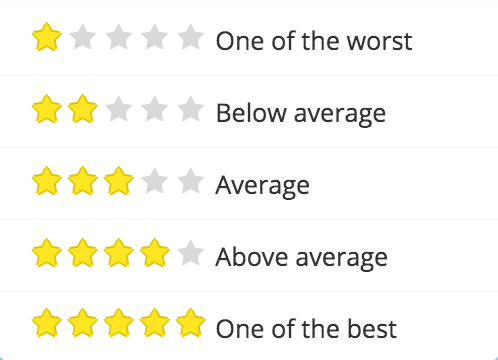
\includegraphics[width=0.5\textwidth]{datamodel-reviews}
\caption{Course and opportunity review ratings.}
\end{figure}

\subsection{Roles}
Roles represent the different user roles allowed in RadGrad. There are currently six roles: faculty, student, admin, alumni, advisor, and mentor. Currently, users are allowed to have exactly one role. All users except for admin and advisor can view only their own RadGrad pages. Advisors can also view student RadGrad pages, and admin can view all RadGrad pages. 

\subsection{Semesters}
Semesters represent an academic semester at the University of Hawaii. Each semester has an associated term, year, number to sort by, semester number, and slug. There are three possible terms: Spring, Summer, and Fall. The number to sort by easily allows chronological comparisons between semesters. Semester number is used for ??? 

\subsection{Slugs}
Slugs are strings used as part of a URL to uniquely identify an entity. These strings do not change with different instantiations of the database like docIDs do. Slugs are used in the RadGrad data model to represent relationships between different entities. Therefore, only collections that need to be referenced by other collections contain a slug. 

\subsection{Teasers}
Teasers represent short videos that advertise an ICS opportunity. Each teaser has an associated title, slug, author, URL, description, duration, related interests, and opportunity. Any member of RadGrad can be an author of a teaser. Teasers are typically less than a minute long and function as a sort of quick advertisement to get potential students interested in participating in that particular opportunity. 

\subsection{Users}
Users represent anyone who has created an account on the RadGrad system. Each user has an associated username, first name, last name, slug, email, password, UH ID, career goals, interests, desired degree, picture, level, website, hidden courses, and hidden opportunities. The user's RadGrad username is the same as their UH email name. This, along with their email, cannot be changed once the user's account is created. Only student users will have a desired degree and a level. Hidden courses and hidden opportunities are used to keep track of courses and opportunities that students have actively ``hidden" from their page. By keeping track of these hidden courses and opportunities, students can have the option to make them visible again.

\subsection{Verification Requests}
Verification requests represent a request from a student to get verification and ICE points for completing an opportunity. Each opportunity has an associated date, status, verifier, and feedback. There are three possible statuses: accepted, rejected, and open. The verifier is the user who has verified the event. Only advisors, faculty, and admin can be a verifier. If a request is rejected, the verifier can add reasons for the rejection in the feedback field. The student can then see the feedback and the results of the verification. If the verifier wishes to reopen the verification request, they may do so at any time. A student who would like to reopen a request will need to contact the verifier.  

\subsection{Academic Years}
Academic years represent an academic year at the University of Hawaii. Each academic year has an associated year, spring year, student, and semesters. Since academic years start in the Fall and end in the Summer, they span two years: year, and spring year. A student on RadGrad must have an academic year for each year, or portion of a year, that they are enrolled in an ICS course or participated in an ICS opportunity.

\section{Testing}
\subsection{Interactive Testing}
RadGrad uses interactive server-side testing with Mocha test runner and Chai Expect Assertions during code production in order to maintain correctness. Each collection class from the data model has tests in a corresponding sibling file. These tests include checking if a new collection entity can be defined, if a collection entity can be removed, if a collection entity can be dumped from the database, and if a collection entity can be restored from a dump file to the database.     

\subsection{Personas}
\subsection{Beta Testing}
\subsubsection{Student Beta Testing}
\subsubsection{Advisor Beta Test}

\section{Student Mode}
\subsection{Degree Planner}
\subsubsection{Degree Planner}

\subsubsection{Recommendations and Warnings}

\subsubsection{Career Goal, Course, Desired Degree and Opportunity Explorers}
\begin{figure}[h]
\centering
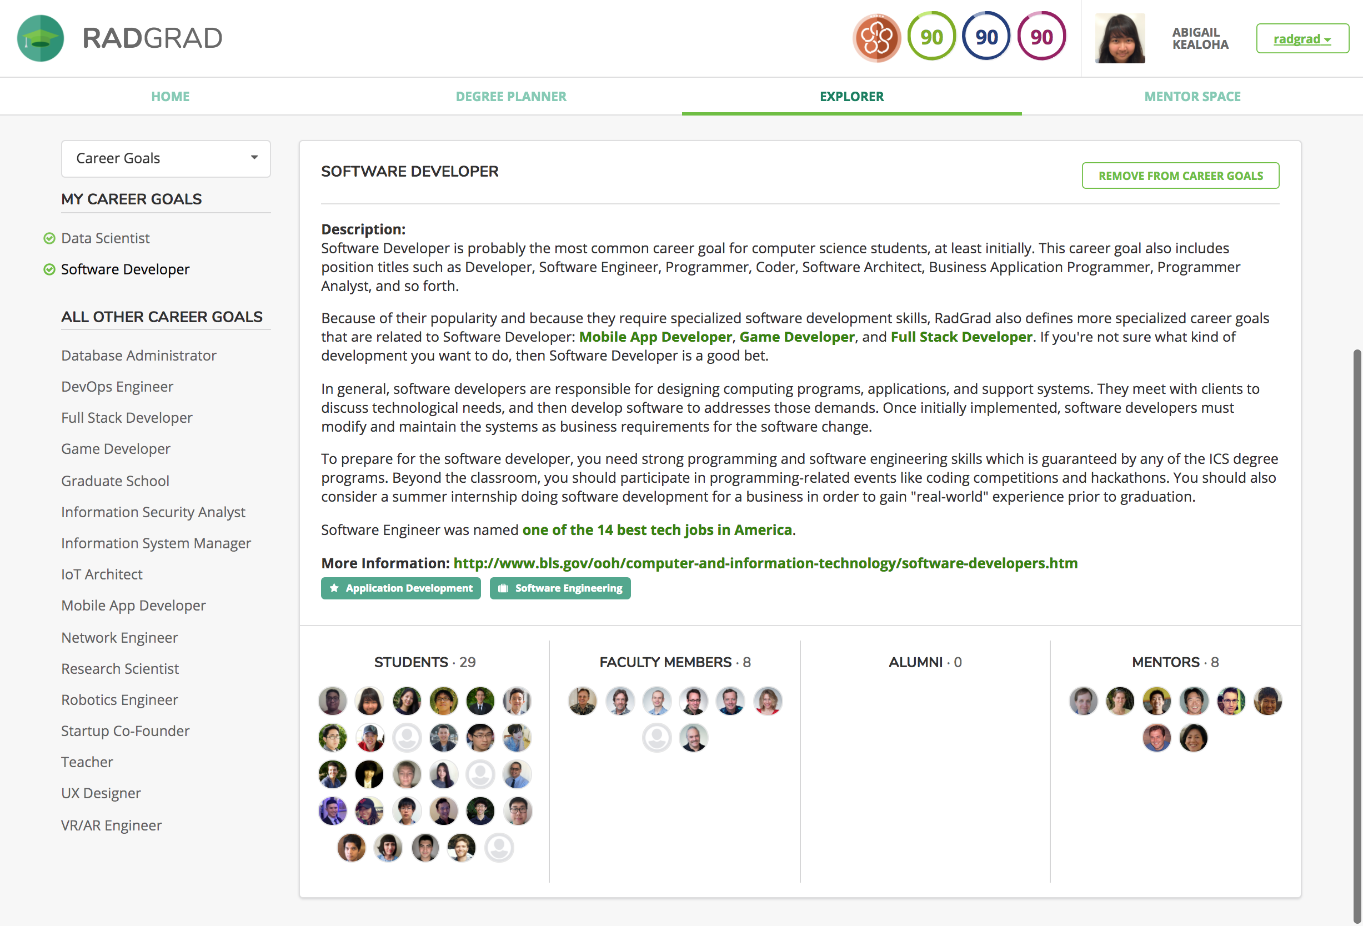
\includegraphics[width=1.0\textwidth]{careergoal-explorer}
\caption{Career Goal Explorer page.}
\end{figure}

Students can access the career goal, course, desired degree, and opportunity explorers to help them plan their degree.  These explorers can be accessed through the ``Explorer" top menu on the student home page. The specific explorer can be chosen using the dropdown menu on the left side. 

The career goal explorer lists all RadGrad career goals on the left side. These career goals are arranged by ``My Career Goals" (career goals that the user has added) and ``All other career goals" (career goals that the user has not added). The user can click on a career goal to view details about that career goal. These details include a description of the career goal, related interests, related courses and/or opportunities, a link for more information, interested students, interested faculty, interested alumni, and interested mentors. On this page, the student can also add or remove the career goal by clicking on the green button at the top right corner.  

The course explorer lists all RadGrad courses on the left side. These courses are arranged by ``Courses in my Plan" (all part, present or future courses in the student's degree plan) and ``All Other Courses."  

\subsubsection{Teasers}

\subsection{Social Network}
\subsubsection{Avatars}

\subsubsection{Feed}

\subsubsection{Mentorspace}

\subsubsection{Advisor Log}

\subsubsection{Reviews}

\subsubsection{User Explorer}

\subsection{Gamification}
\subsubsection{ICE}

\subsubsection{Levels}

\section{Advisor Mode}

\section{Administrator Mode}